Après quelques tentatives infructueuses pour porter le noyau linux sur le matériel, la création d'un noyau minimal semblait être un bon compromis car pour utiliser le \textit{PR}, même un noyau basique voire pas de noyau aurait pu suffir.

\subsection{Ses fonctionnalités}

Le noyau qui a été développé en \languagetoto{C++} gère des mécanismes minima. Il permet d'utiliser l'UART pour dialoguer avec l'utilisateur. Un tas a été créé pour permettre l'allocation dynamique de mémoire. Il est possible de paramétrer sa position et sa taille en mémoire.\\
Un driver de VGA a été entrepris mais non terminé puisque le VGA n'est pas tout à fait fonctionnel.\\
Ce noyau gère aussi les interruptions matérielles comme la réception d'un octet sur l'UART et les interruptions des timers.
Un des timers génère une interruption périodique réglable qui pourrait être utilisée pour du \english{multitasking}.\\
Actuellement, aucun appel système n'est géré mais ils peuvent être implémentés aisément.

\subsection{Un pseudo-terminal}

Le pseudo-terminal a été développé en \languagetoto{C} et a pour but de permettre à l'utilisateur de lancer un programme présent en mémoire flash. Le fichier de configuration contient plusieurs lignes associant des informations (adresse en flash et taille) à un programme. Il a aussi pour but de pallier au manque de système de fichiers. En effet, le programme récupère ses informations dans un fichier de configuration présent à une adresse fixe en flash. Lorsque l'utilisateur entre une commande dans le pseudo-terminal, ce dernier va parcourir le fichier de configuration pour trouver les informations associées à la commande entrée par l'utilisateur. Si le nom demandé n'est pas trouvé, une erreur est affichée. Sinon il devra demander au noyau de charger le programme en RAM et de l'exécuter. Cette dernière partie n'a pas été implémentée puisque l'appel système \texttt{malloc} nécessaire pour la comparaison des noms de programme n'a pas été implémenté.

\subsection{Affichage sur la sortie VGA}

Les données à destination de la sortie VGA sont stockées en RAM à une adresse paramétrable. La fréquence de lecture de la mémoire vidéo se fera à la fréquence de rafraîchissement du VGA. Quant à l'écriture, elle ne sera pas périodique et ne surviendra que lors d'une modification de contenu : lorsqu'on tape au clavier, lors d'un affichage de message sur la sortie standard. Il serait possible d'afficher des images au format Bitmap directement sur le SoC en les convertissant au bon format pour être lisible par le VGA.

\begin{figure}[h!]
\centering
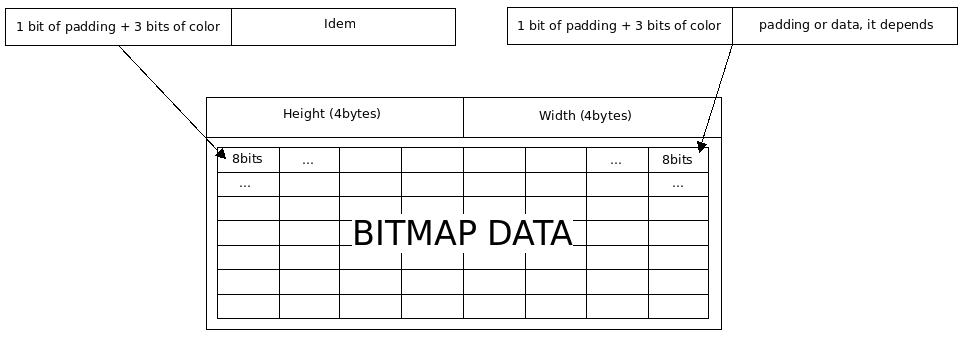
\includegraphics[scale=0.4]{formatBmpFile.png}
\caption{Format du fichier lisible par le VGA}
\label{format-bitmap-vga}
\end{figure}

La mémoire vidéo récupèrera les données du pseudo-format présenté sur la figure \ref{format-bitmap-vga}. La sortie VGA de la \nexys{} ne supporte que 3 bits de couleurs. Nous nous sommes donc contentés de mettre dans l'en-tête du fichier la largeur et la longueur en pixel de l'image, qui sont des informations suffisantes pour déduire par la suite la taille totale de l'image. Cela implique tout de même qu'il faudra faire attention à la taille totale de l'image pour ne pas déborder dans une autre zone de la RAM. Puis s'enchaînent les données dans le format présenté sur la figure \ref{format-bitmap-vga}. Un pixel sera codé sur 3 bits. Il y aura donc 2 pixels par octets et également 2 bits de padding. Il y aura un éventuel padding pour les lignes de pixel pour réaliser un alignement sur 8 bits.

\subsection{Le driver pour l'Ethernet}

Le code du driver a été trouvé comme dit précédemment sur un \href{http://svn.ohwr.org/lm32/crt/mac/}{SVN}. Les parties en assembleur dans le code ne sont pas à réécrire (compatible avec le LM32). Cependant, nous n'avons pas eu le temps de le tester. Il faudrait, pour commencer, regarder les exemples d'utilisation fournis et réaliser un test simple.\\
Plusieurs fonctions tels que \texttt{memcpy}, \texttt{memcmp} ou encore diverses fonctions d'affichage ont été définies pour une autre plateforme. Il faudrait les intégrer à ce qui existe déjà dans notre \english{library} ainsi que le \english{handler} d'interruption.\\
Dans l'état actuel, si on se penche sur les services déjà implémentés, il y a une fonction pour initialiser le module, le désactiver, envoyer et recevoir des données et enfin mettre en place un \english{handler} pour l'interruption associée à la réception de données.

